\documentclass[11pt]{article}
\usepackage[margin=0.82in]{geometry}
\usepackage[T1]{fontenc}
\usepackage{lmodern}
\usepackage{microtype}
\usepackage{amsmath,amssymb,mathtools}
\usepackage{graphicx}
\usepackage{booktabs}
\usepackage{tabularx}
\usepackage{array}
\usepackage{float}
\usepackage{enumitem}
\usepackage{caption}
\usepackage{xcolor}
\usepackage{hyperref}
\usepackage[backend=biber,style=numeric,natbib=true,sorting=none]{biblatex}
\addbibresource{paper.bib}
\usepackage{multirow}
\hypersetup{colorlinks=true,linkcolor=blue!45!black,citecolor=blue!45!black,urlcolor=blue!45!black,pdftitle={Interrogating Alien Life: Adversarially Trained Reinforcement Learning for Substrate-Agnostic Detection of Self-Repair Dynamics},pdfauthor={Devanik Debnath}}
\graphicspath{{figures/}}
\setlength{\parskip}{0.35em}
\setlength{\parindent}{0pt}
\captionsetup{font=small,labelfont=bf}
\setlist{itemsep=0.15em,topsep=0.2em}
\newcommand{\R}{\mathcal{R}}
\newcommand{\A}{\mathcal{A}}
\newcommand{\Hrep}{H_{\mathrm{rep}}}
\newcommand{\Habi}{H_{\mathrm{abi}}}
\newcommand{\clip}{\operatorname{clip}}

\title{\vspace{-1.2em}\textbf{Interrogating Alien Life: Adversarially Trained Reinforcement Learning for Substrate-Agnostic Detection of Self-Repair Dynamics}}
\author{Devanik Debnath\\\small Independent research preprint; author profile: \href{https://github.com/Devanik21}{Devanik21}}
\date{17 October 2026}

\begin{document}
\maketitle

\begin{abstract}
A search for life that presupposes terrestrial molecules or familiar morphology risks missing unfamiliar systems, yet broad dynamical traits such as recovery after damage are not unique to biology. We propose an intervention-based framework for evaluating self-repair-like dynamics without requiring a particular chemical substrate. A sensor policy selects among five bounded probes: initial recovery, dependence on an external drive or gradient, response to repeated perturbation, spatial localization, and transfer to a novel perturbation context. A finite family of synthetic abiotic decoys---passive relaxation, self-healing material, driven oscillator, and scripted controller---acts as a deliberately confounding null set. A tabular reinforcement-learning policy is trained with adaptive hard-negative reweighting, which shifts training probability toward decoys that currently trigger false positives. In one fixed-seed synthetic benchmark, adversarial Q-learning reaches 0.935 balanced accuracy and 0.979 score AUROC while using an average of 3.75 probes; its worst-decoy false-positive rate is 0.168, versus 0.244 for uniformly trained Q-learning and 0.328 for a fixed five-probe likelihood-ratio panel. A recovery-only baseline has 0.746 worst-decoy false-positive rate, illustrating why recovery alone is weak evidence. A one-factor noise sweep reduces balanced accuracy from 0.975 at 0.75 times nominal noise to 0.848 at 1.5 times nominal noise. These are results from hand-specified synthetic worlds, not observations from planetary samples or proof of extraterrestrial life. The contribution is a falsifiable assay design and reproducible computational baseline; empirical transfer across substrates and instruments remains untested.
\end{abstract}

\textbf{Keywords:} agnostic biosignatures; astrobiology; self-repair; active sensing; adversarial reinforcement learning; hard-negative mining; nonequilibrium dynamics; false-positive control

\section{Introduction}
How should an instrument interrogate a system when the target substrate is unknown, but the system can be perturbed and observed over time? A conventional life-detection pipeline often starts from specific chemical, isotopic, morphological, or atmospheric signals. Agnostic biosignature research broadens that search by asking what observations may be informative without assuming a familiar terrestrial molecular inventory \citep{Graham2026Agnostic,Cleaves2023MLBiosignature}. Mission-oriented frameworks also stress contextual interpretation, ambiguity, and false-positive analysis rather than a single decisive feature \citep{Neveu2018Ladder,Malaterre2023Biosignature,Walker2018Exoplanet}.

This paper asks whether a more active strategy is useful: instead of merely observing a candidate system, select small, bounded perturbations and compare the resulting response with competing abiotic explanations. The focal pattern is *self-repair-like dynamics*: a localized disturbance is reduced, the response may depend on available drive or resources, repeated insults may reveal state or history dependence, and activity may cease or change once the disturbance has been resolved. These operational features are inspired by known biological repair and nonequilibrium organization, but none is assumed to be unique to life. Biological tissue models can display self-healing trajectories, while nonliving materials and driven processes can also relax or recover \citep{Suki2020SelfHealing,Youk2026NonEquilibrium}.
The core danger is a false inference: if a system returns toward a baseline, it may be a passive relaxor, a synthetic self-healing material, a driven oscillator, or an engineered controller. The proposed method therefore treats those mechanisms as explicit hard negatives. Reinforcement learning (RL) chooses which measurements to acquire under a probe budget; adversarial hard-negative sampling makes the policy face the most confusing decoy families encountered during training. Adversarial RL has prior methodological precedent in other detection settings, so novelty is not claimed for adversarial RL itself \citep{Tong2020AdversarialRL}.

\textbf{Contributions.} This preprint contributes (i) an operational, substrate-agnostic framing for a repair-response assay; (ii) a finite-horizon active-probing formulation with five normalized response tests; (iii) a reproducible synthetic benchmark with four abiotic decoy families, a uniform-training RL control, and fixed-policy baselines; and (iv) explicit failure criteria for moving from simulation toward terrestrial analogue experiments. It does not claim a universal biosignature, a validated alien-life detector, or a new theorem about the nature of life.

\section{Related work and bounded novelty claim}
The literature contains several adjacent foundations. The 2026 review by Graham summarizes attempts to search for life without assuming Earth-like molecular or metabolic signals \citep{Graham2026Agnostic}. Cleaves and colleagues report a machine-learning approach using relational structure in pyrolysis--gas chromatography--mass spectrometry data, demonstrating that multivariate measurement patterns can carry information beyond the identification of individual compounds \citep{Cleaves2023MLBiosignature}. This is a chemical-sample result, not evidence for our intervention-based features. NASA's Ladder of Life Detection provides criteria for interpreting measurements under robotic-mission constraints and explicitly leaves room for community revision \citep{Neveu2018Ladder}. The biosignature concept itself has been critically examined because causal interpretations can be more ambiguous than the label suggests \citep{Malaterre2023Biosignature}.

Two additional connections shape the method. First, formal self-healing models demonstrate that return-to-baseline behavior can arise from state-dependent interaction mechanisms and network dynamics \citep{Suki2020SelfHealing}. Second, non-equilibrium-capacity discussions distinguish a system's instantaneous state from its capacity to resume organized dynamics \citep{Youk2026NonEquilibrium}. Both motivate measuring response under controlled changes, not treating one trajectory as a universal criterion. Finally, adversarial RL has been developed for detection tasks in other fields \citep{Tong2020AdversarialRL}; its use here is a transfer of method, not evidence of performance in astrobiology.

\begin{table}[htbp]
\centering\small
\caption{Selected literature and the narrow role each source plays in this proposal.}
\label{tab:literature}
\begin{tabularx}{\linewidth}{p{0.22\linewidth}p{0.27\linewidth}X}
\toprule
Source & Established scope & Relevance and boundary \\
\midrule
Graham (2026) \citep{Graham2026Agnostic} & Review of agnostic biosignature concepts & Motivates functional, non-Earth-specific reasoning; does not establish repair as life-specific. \\
Cleaves et al. (2023) \citep{Cleaves2023MLBiosignature} & ML over molecular mass-spectral patterns & Supports multivariate relational analysis; uses a different measurement modality and dataset. \\
Neveu et al. (2018) \citep{Neveu2018Ladder} & Mission-aware life-detection criteria & Supports explicit ambiguity and false-positive accounting. \\
Malaterre et al. (2023) \citep{Malaterre2023Biosignature} & Conceptual analysis of biosignature claims & Motivates restrained causal language and context-sensitive attribution. \\
Suki et al. (2020) \citep{Suki2020SelfHealing} & Analytic and network model of tissue self-healing & Shows repair-like trajectories are modelable, not that they uniquely imply life. \\
Tong et al. (2020) \citep{Tong2020AdversarialRL} & Adversarial RL for detection/alert prioritization & Methodological precedent outside astrobiology; no performance transfer assumed. \\
\bottomrule
\end{tabularx}
\end{table}

The scoped gap is not a claim that no earlier work studies activity-based biosignatures or adversarial active sensing. It is the lack, within the reviewed and bounded search, of an established validation showing that a sequential RL policy can discriminate a repair-response phenotype from an adversarial finite family of abiotic recovery mechanisms across unknown substrates. That gap is a motivation for a benchmark, not a demonstrated absence from the entire literature. The search was not a systematic review or a patent survey.

\section{Operational question and observables}
Let a system with unknown substrate label $s$ have a latent state $x_t$, a controllable perturbation $u_t$, an external drive or gradient proxy $r_t$, and observation channel $m$. A general observation model is
\begin{align}
 x_{t+1} &= F_s(x_t,u_t,r_t,\eta_t), \label{eq:dynamics}\\
 y_t^{(m)} &= H_s^{(m)}(x_t)+\epsilon_t^{(m)}, \label{eq:observation}
\end{align}
where $F_s$ and $H_s^{(m)}$ are unknown, while $\eta_t$ and $\epsilon_t^{(m)}$ represent process and measurement noise. The substrate-agnostic aspiration is to compare functions of response, not to pretend that units, sensor physics, or state spaces are identical. A practical deployment would need modality-specific normalization and an instrument model; this preprint tests only a dimensionless toy representation.

We define five candidate probes, each returning a scalar synthetic feature scaled approximately to $[0,1]$. The values are *not* measured biological quantities and should not be used as instrument specifications.

\begin{table}[htbp]
\centering\small
\caption{Operational probe set. Every feature has plausible abiotic analogues.}
\label{tab:probes}
\begin{tabularx}{\linewidth}{p{0.17\linewidth}p{0.31\linewidth}X}
\toprule
Probe & Measurement question & Major confounder \\
\midrule
Initial recovery & How much of a localized perturbation dissipates over the observation window? & Passive relaxation can mimic recovery. \\
Drive/gradient gate & Does the response change when an available drive or gradient is altered? & Driven materials and oscillators also depend on external power. \\
Repeated-pulse history & Does the second response depend on the first insult or recovery state? & Hysteretic materials and controllers can store history. \\
Spatial locality & Is the response concentrated near the disturbance and then propagated or confined? & Fracture healing and material transport can be localized. \\
Novel-context transfer & Does the response generalize to a randomized perturbation and stop/change when no repair is needed? & Programmed controllers may mimic a limited test suite. \\
\bottomrule
\end{tabularx}
\end{table}

An interpretable repair-response hypothesis, $\Hrep$, predicts a coordinated pattern across some subset of these probes. The composite abiotic hypothesis, $\Habi$, includes any nonliving mechanism capable of producing a subset of the pattern. A positive score therefore means "more consistent with the specified repair-capable simulator than with the specified decoy family," not "life detected." Substrate agnosticism is a research objective that requires cross-modal validation; a common dimensionless feature vector is not by itself proof of invariance.

\section{Sequential probe selection}
Let the available action set be $\A=\{a_1,\ldots,a_5\}$, corresponding to Table~\ref{tab:probes}. Each test can be used at most once in an episode. Let $m_t\in\{0,\ldots,31\}$ encode previously used probes and $e_t\in[-8,8]$ denote a clipped accumulated evidence score. For a measurement $z$ under action $a$, the simulator defines a Gaussian repair density
\begin{equation}
 p_R(z\mid a)=\mathcal{N}(z;\mu_{R,a},\sigma_a^2),
 \label{eq:repairdensity}
\end{equation}
and a finite abiotic mixture
\begin{equation}
 p_A(z\mid a;w)=\sum_{j=1}^{J}w_j\,\mathcal{N}(z;\mu_{j,a},\sigma_a^2),\qquad \sum_{j=1}^{J}w_j=1.
 \label{eq:abidensity}
\end{equation}
Here $J=4$. The score increment and state transition are
\begin{align}
 \ell_a(z;w)&=\log p_R(z\mid a)-\log p_A(z\mid a;w),\label{eq:llr}\\
 e_{t+1}&=\operatorname{clip}(e_t+\ell_{a_t}(z_t;w),-8,8).\label{eq:evidence}
\end{align}
This is a log-density ratio under the stated synthetic Gaussian family. It is not a universally calibrated probability. At each step the policy chooses an unused probe or a stop action, "repair-like" or "not repair-like." The finite-horizon state is $s_t=(m_t,b(e_t))$, where $b$ maps clipped evidence to one of 31 bins. The Q table has shape $32\times31\times7$.

The immediate probe reward is $-0.035$. At stopping, correct classification receives $+1$, a false positive receives $-1.6$, a false negative receives $-1$, and an additional $-0.02$ is charged per probe used. The false-positive penalty is deliberately higher than the false-negative penalty, but this is a design choice rather than a mission-certified loss function. Q-learning uses discount factor $\gamma=0.96$, learning rate $\alpha=0.18$, and an exploration probability decaying from $0.30$ to a floor of $0.035$. Each observed transition is updated online and revisited once in reverse order after the episode's terminal decision.

\section{Adversarial hard-negative training}
A separate adversarial policy is not solved to a formal game-theoretic equilibrium. Instead, every 5,000 training episodes, the current greedy detector is evaluated against each abiotic family using 100 generated episodes per family. Estimated false-positive rates $f_j$ are transformed into weights
\begin{equation}
 \widetilde w_j=\frac{\exp(5f_j)}{\sum_k\exp(5f_k)},\qquad
 w_j=0.65\widetilde w_j+0.35/J. \label{eq:weights}
\end{equation}
Future negative training episodes are sampled according to $w$. The retained uniform component prevents the sampler from completely dropping any decoy family. This is adaptive hard-negative reweighting inspired by adversarial training; it is not a learned adversary optimizing an arbitrary observation-generating mechanism, and its claims should not be extended beyond the finite decoy set.

\begin{figure}[htbp]
\centering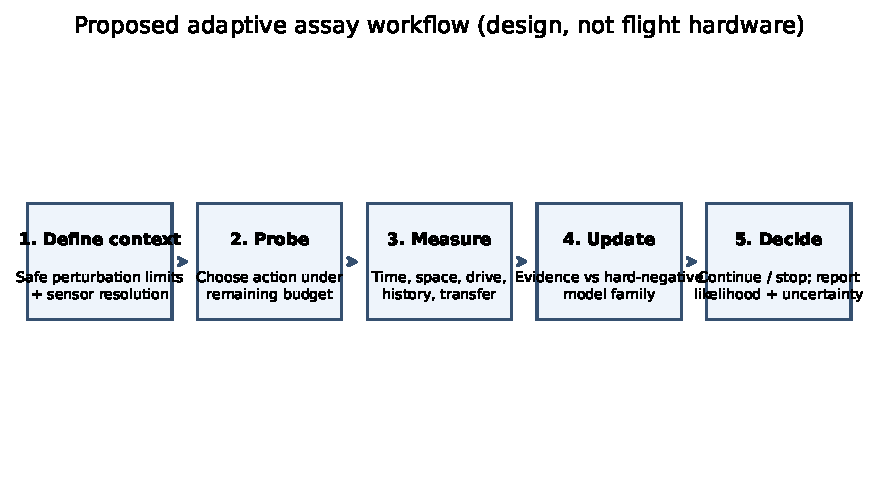
\includegraphics[width=0.98\linewidth]{fig7_method_flow.pdf}
\caption{Proposed adaptive assay sequence. Perturbation safety and instrument-specific operating limits must be established before real-world use.}
\label{fig:method}
\end{figure}
\begin{figure}[htbp]
\centering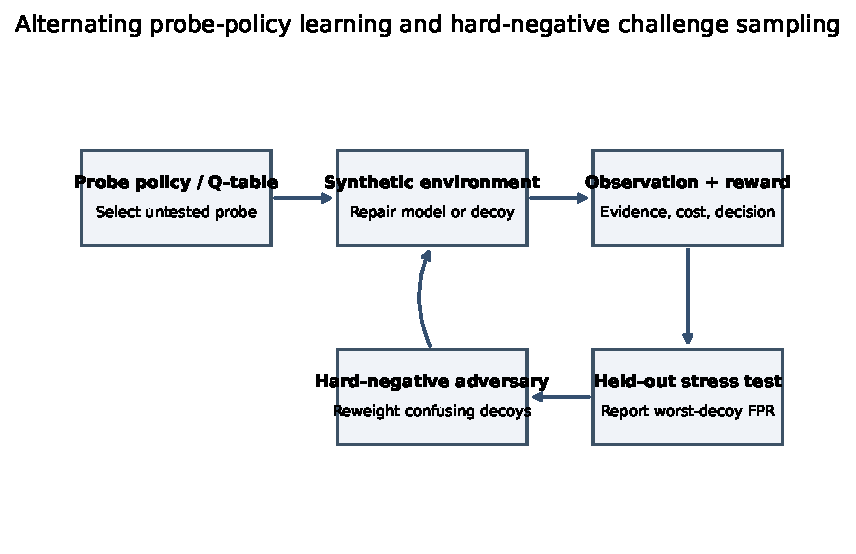
\includegraphics[width=0.98\linewidth]{fig8_adversarial_training.pdf}
\caption{Training loop: a finite synthetic challenge family is used to reweight confusing abiotic worlds. The diagram represents the present implementation, not a general minimax guarantee.}
\label{fig:training}
\end{figure}

\section{Synthetic benchmark}
\subsection{Worlds and parameters}
The benchmark contains one repair-capable synthetic world and four abiotic decoy families: passive relaxor, self-healing material, driven oscillator, and scripted controller. All observations are generated by Gaussian draws around hand-specified means and clipped to $[-0.15,1.15]$. Table~\ref{tab:parameters} gives the means; the probe-specific noise standard deviations are $(0.12,0.13,0.14,0.13,0.14)$ at nominal noise. The parameter values encode qualitative relationships by construction and are not estimated from any physical or biological dataset. The exact parameter file is archived in \texttt{results/challenge\_world\_parameters.csv} and the generator is \texttt{verify\_model.py}.

\begin{table}[htbp]
\centering\scriptsize
\caption{Synthetic mean response values by probe. All entries are illustrative model parameters, not observations.}
\label{tab:parameters}
\resizebox{\linewidth}{!}{%
\begin{tabular}{lrrrrr}
\toprule
World & Initial recovery & Drive gate & History & Locality & Context transfer \\
\midrule
Repair-capable & 0.78 & 0.72 & 0.69 & 0.75 & 0.71 \\
Passive relaxor & 0.82 & 0.18 & 0.22 & 0.30 & 0.24 \\
Self-healing material & 0.84 & 0.48 & 0.42 & 0.78 & 0.44 \\
Driven oscillator & 0.56 & 0.74 & 0.28 & 0.50 & 0.25 \\
Scripted controller & 0.77 & 0.62 & 0.64 & 0.68 & 0.39 \\
\bottomrule
\end{tabular}}
\end{table}

The scripted controller is intentionally difficult: it reproduces several repair-like means while weakening novel-context transfer. This is not a claim that real abiotic systems follow these distributions; it is a transparent stress case designed to prevent a recovery-only detector from trivially succeeding. Figure~\ref{fig:recovery} visualizes the central confound: recovery curves can be close even when the generating mechanism differs.

\begin{figure}[htbp]
\centering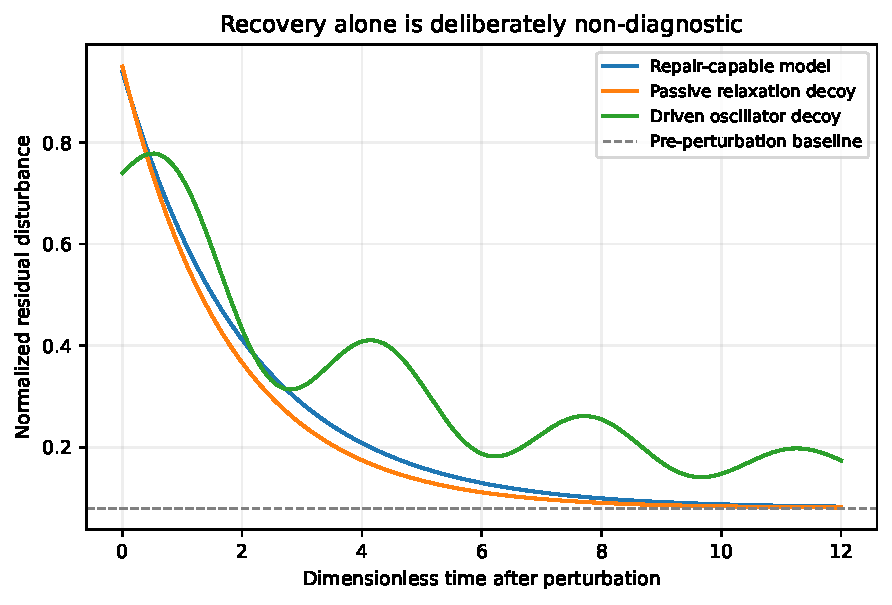
\includegraphics[width=0.90\linewidth]{fig3_recovery_confounds.pdf}
\caption{Synthetic normalized residual-disturbance curves. The repair-capable and passive-relaxation curves deliberately overlap; their similarity is a counterexample to interpreting recovery alone as life-specific.}
\label{fig:recovery}
\end{figure}

\subsection{Training and evaluation protocol}
The fixed random seed is 20261017. Each RL variant receives 30,000 training episodes. At evaluation, each method is assessed on 500 repair-capable episodes and 500 episodes from each of the four abiotic families, for 2,500 episodes per method. These are held-out random draws but not held-out mechanisms, parameter shifts, or sensor modalities. We compare:
\begin{enumerate}
\item \textbf{Adversarial Q-RL}: adaptive hard-negative weighting described above.
\item \textbf{Uniform Q-RL}: identical Q-learning procedure with equal decoy weights throughout training.
\item \textbf{Recovery-only}: one initial-recovery measurement, thresholded at the midpoint between the repair mean and the average decoy mean for that probe.
\item \textbf{Fixed full panel}: all five probes and a zero-threshold sum of uniform-mixture log-likelihood increments.
\item \textbf{Random-order panel}: the same five-probe score, measured in randomized probe order.
\end{enumerate}

The primary classification metrics are sensitivity, specificity, balanced accuracy, and worst-decoy false-positive rate (FPR). Score AUROC compares the cumulative likelihood-ratio score across positive and negative episodes and is reported as a ranking metric, not as calibrated probability. Wilson 95\% intervals are computed for binomial sensitivity/specificity/FPR. These intervals quantify episode-sampling uncertainty conditional on this simulator and fixed training seed; they do not quantify training-seed variation, parameter uncertainty, or model misspecification.

\section{Results}
\subsection{Main benchmark}
The adversarial Q-RL agent reaches sensitivity $0.932$, specificity $0.938$, balanced accuracy $0.935$, and score AUROC $0.979$, using an average of 3.75 probes. The aggregate FPR is $0.0625$ with Wilson 95\% interval $[0.0527,0.0740]$. Its worst-decoy FPR is $0.168$ against the scripted controller, with a decoy-specific Wilson interval $[0.1378,0.2033]$. Uniform Q-RL achieves a slightly higher AUROC of $0.983$ and sensitivity of $0.942$, but its worst-decoy FPR is $0.244$. The fixed panel achieves high sensitivity ($0.976$) but its worst-decoy FPR is $0.328$ and it always spends five probes. On this one benchmark, adaptive hard-negative training improves the most difficult decoy's observed FPR at the cost of a modest decrease in sensitivity relative to uniform Q-RL and a greater average probe count. No significance claim is warranted from this single training seed.

\begin{table}[htbp]
\centering\scriptsize
\caption{Held-out synthetic episode metrics. Each method has 500 positive episodes and 500 episodes from each of four negative families.}
\label{tab:mainresults}
\resizebox{\linewidth}{!}{%
\begin{tabular}{lrrrrrr}
\toprule
Method & Sensitivity (95\% Wilson CI) & Specificity & Balanced accuracy & AUROC & Worst-decoy FPR & Mean probes \\
\midrule
Adversarial Q-RL & 0.932 (0.906--0.951) & 0.938 & 0.935 & 0.979 & 0.168 & 3.75 \\
Uniform Q-RL & 0.942 (0.918--0.959) & 0.919 & 0.931 & 0.983 & 0.244 & 3.51 \\
Recovery-only & 0.552 (0.508--0.595) & 0.496 & 0.524 & 0.604 & 0.746 & 1.00 \\
Fixed full panel & 0.976 (0.959--0.986) & 0.876 & 0.926 & 0.983 & 0.328 & 5.00 \\
Random-order panel & 0.972 (0.954--0.983) & 0.895 & 0.933 & 0.984 & 0.288 & 5.00 \\
\bottomrule
\end{tabular}}
\end{table}

\begin{figure}[htbp]
\centering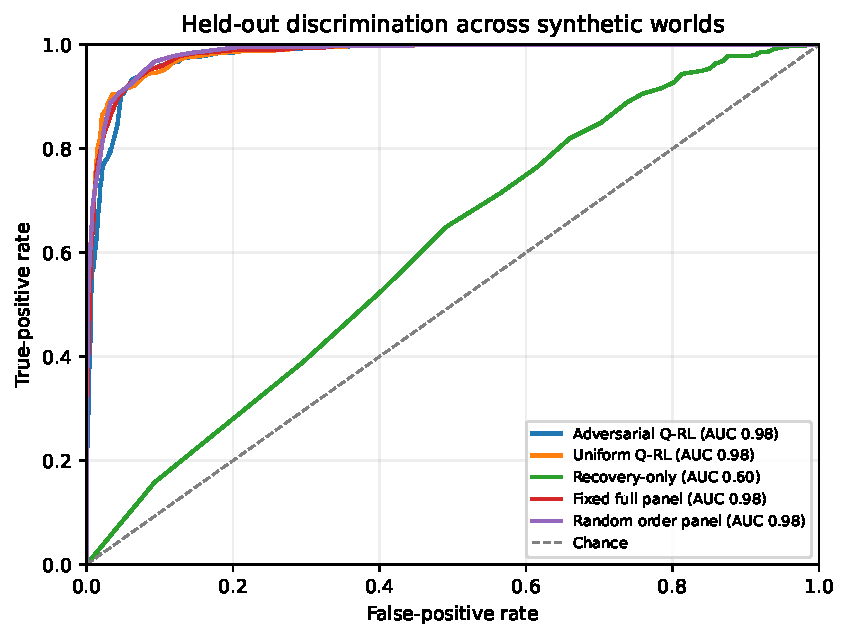
\includegraphics[width=0.92\linewidth]{fig1_roc.pdf}
\caption{ROC curves over held-out samples from the synthetic benchmark. AUROC reflects score ranking under the current generative model and must not be interpreted as field-detection accuracy.}
\label{fig:roc}
\end{figure}

\begin{figure}[htbp]
\centering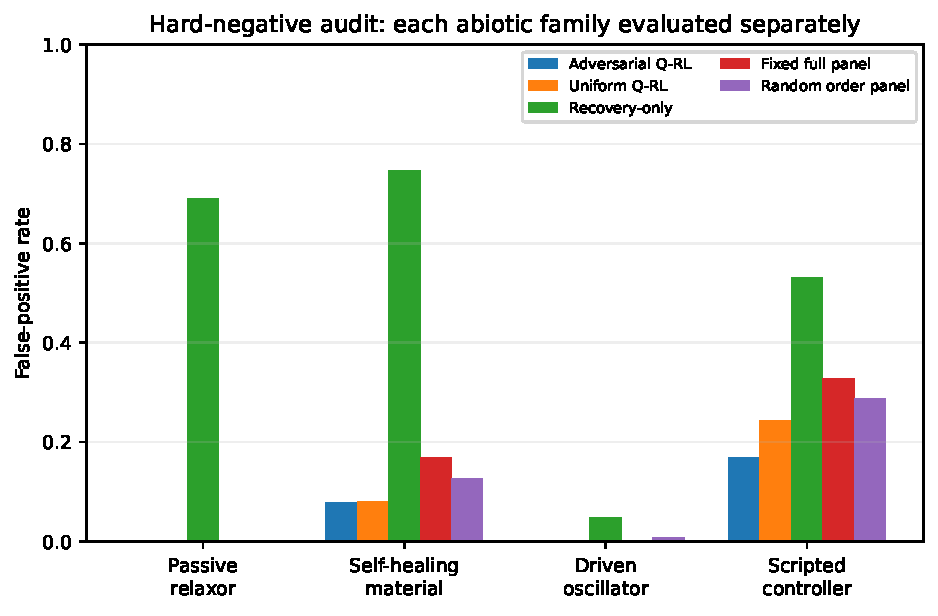
\includegraphics[width=0.98\linewidth]{fig2_decoy_fpr.pdf}
\caption{FPR by abiotic decoy class. The scripted controller is the hardest family for all policies shown; average FPR conceals this failure mode.}
\label{fig:fpr}
\end{figure}

The recovery-only baseline has balanced accuracy $0.524$ and a worst-decoy FPR of $0.746$ because passive relaxation and synthetic self-healing share a high initial-recovery mean with the repair-capable model. This supports a narrow design conclusion: the benchmark requires multiple perturbation-response dimensions to separate the chosen hypotheses. It does not show that these five dimensions are universal or sufficient in nature.

\begin{figure}[htbp]
\centering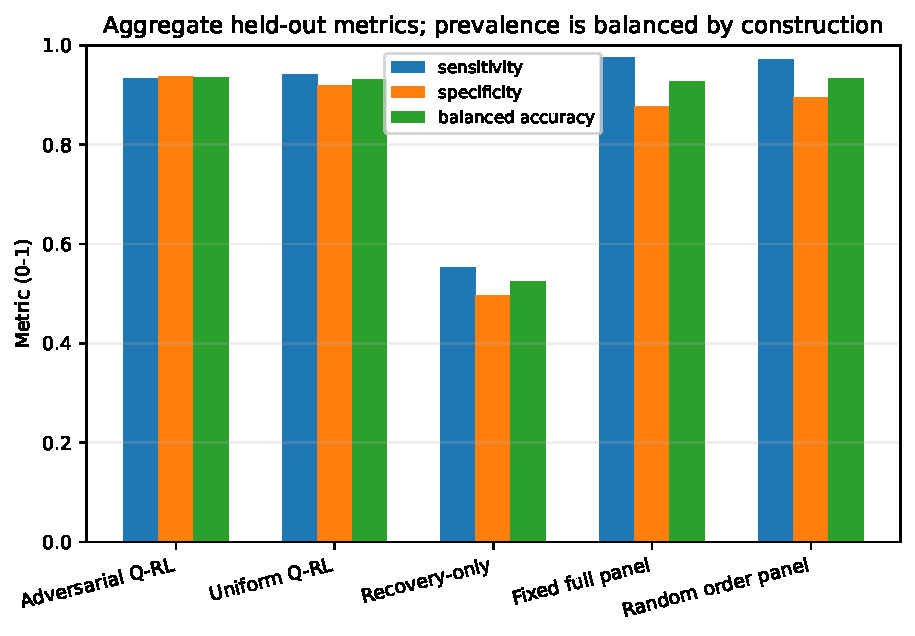
\includegraphics[width=0.92\linewidth]{fig4_metrics.pdf}
\caption{Aggregate held-out metrics. The panel methods sample all five probes; the RL policies can stop early, so the comparison includes a measurement-budget dimension.}
\label{fig:metrics}
\end{figure}

\subsection{Noise sensitivity}
For a one-factor test, the trained adversarial policy was kept fixed while probe noise standard deviations were multiplied by $0.75$, $1.0$, $1.25$, and $1.5$. Each point used 200 positive episodes and 200 episodes from each negative family. Balanced accuracy decreased from $0.975$ at $0.75\times$ noise to $0.848$ at $1.5\times$ noise. The worst-decoy FPR did not vary monotonically because the evaluation is finite and decision outcomes change discretely, emphasizing the need for repeated seeds and larger evaluation sets. The full sweep is archived in \texttt{results/noise\_sensitivity.csv}.

\begin{table}[htbp]
\centering\small
\caption{One-factor noise sensitivity with a fixed learned policy. The nominal-noise point uses 1,000 episodes, whereas the main table uses 2,500; small differences are expected.}
\label{tab:noise}
\begin{tabular}{rrrrr}
\toprule
Noise multiplier & Sensitivity & Specificity & Balanced accuracy & Worst-decoy FPR \\
\midrule
0.75 & 0.980 & 0.970 & 0.975 & 0.085 \\
1.00 & 0.930 & 0.923 & 0.926 & 0.235 \\
1.25 & 0.810 & 0.931 & 0.871 & 0.165 \\
1.50 & 0.775 & 0.921 & 0.848 & 0.210 \\
\bottomrule
\end{tabular}
\end{table}

\begin{figure}[htbp]
\centering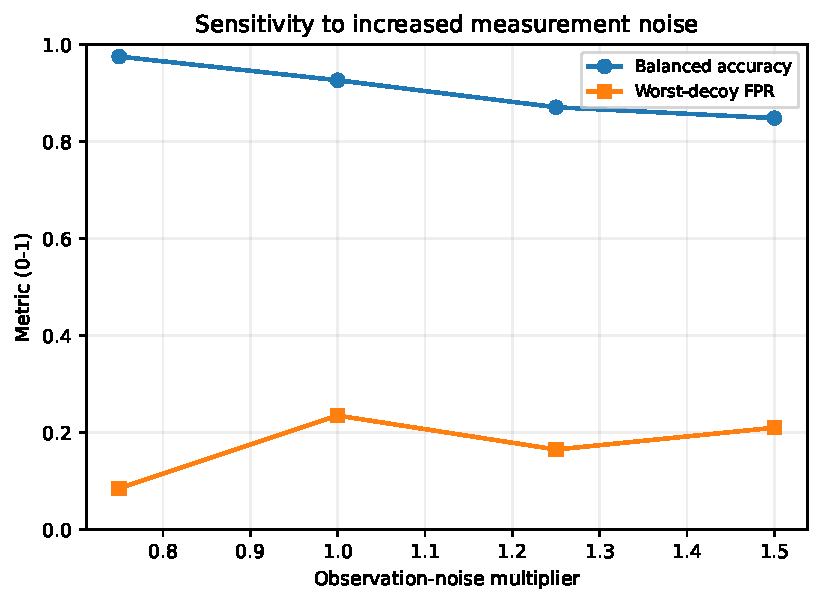
\includegraphics[width=0.88\linewidth]{fig9_noise_sensitivity.pdf}
\caption{Balanced accuracy and worst-decoy FPR as measurement noise changes. The plotted benchmark has one fixed training seed and finite evaluation draws.}
\label{fig:noise}
\end{figure}

\subsection{Measurement and confounding structure}
Figure~\ref{fig:measurementgraph} summarizes the proposed causal measurement flow: controlled perturbations reach a latent system; temporal, spatial, drive-coupling, and transfer observations feed the probe-selection policy. The substrate label is intentionally absent from the policy inputs, but absence of a label is not proof of substrate invariance. Figure~\ref{fig:confounds} depicts feature overlap with confounder families. Recovery overlaps with several abiotic hypotheses, and even locality or history dependence can be mimicked by engineered systems.

\begin{figure}[htbp]
\centering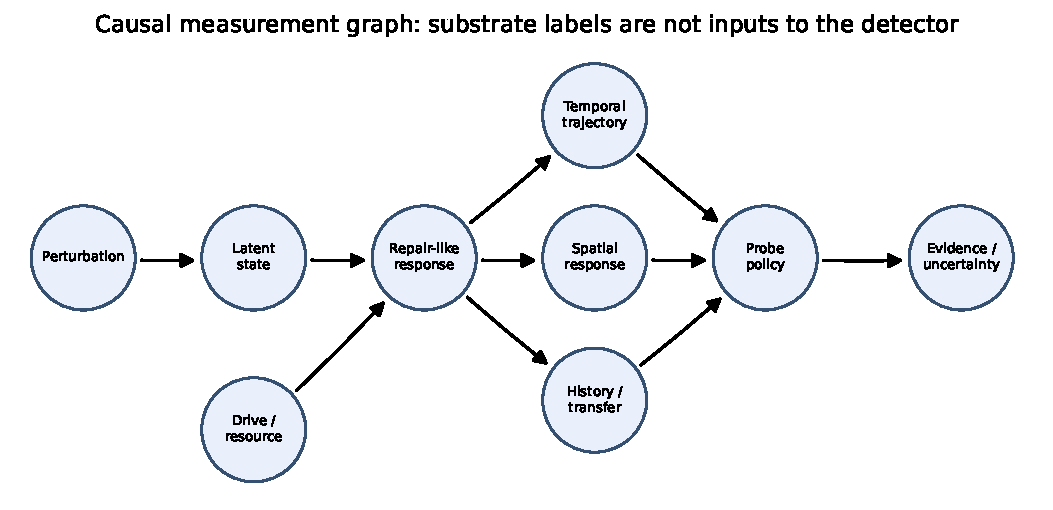
\includegraphics[width=0.98\linewidth]{fig5_measurement_graph.pdf}
\caption{Measurement graph for the proposed assay. It represents a design-level causal abstraction, not a verified causal graph of all living systems.}
\label{fig:measurementgraph}
\end{figure}

\begin{figure}[htbp]
\centering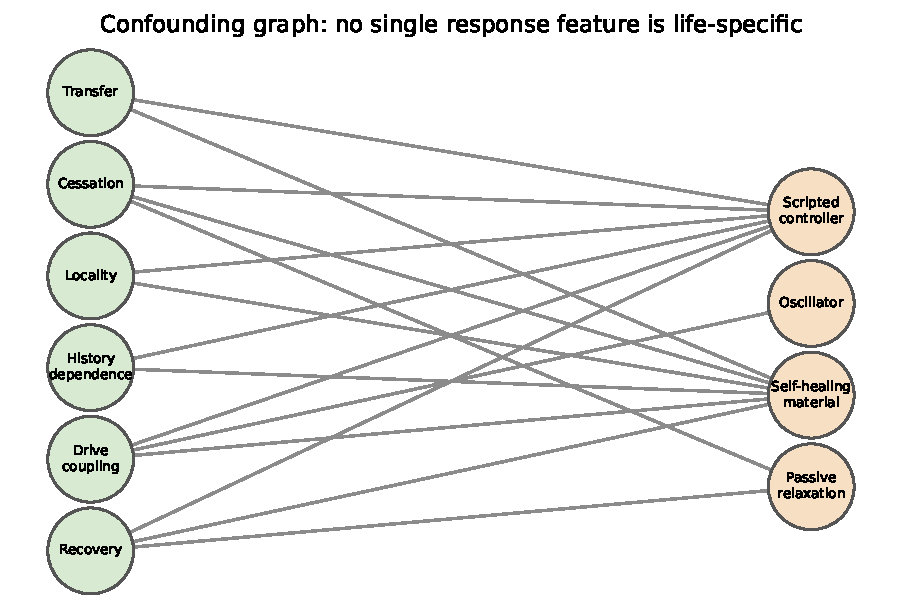
\includegraphics[width=0.91\linewidth]{fig6_confounding_graph.pdf}
\caption{Bipartite graph linking candidate features to plausible abiotic confounders. Edge inclusion expresses a qualitative challenge-design judgement rather than an empirically estimated probability.}
\label{fig:confounds}
\end{figure}

\begin{table}[htbp]
\centering\small
\caption{Main failure modes, falsifiers, and next validation requirements. The future tests below have not yet been run.}
\label{tab:falsification}
\begin{tabularx}{\linewidth}{p{0.23\linewidth}X X}
\toprule
Claim under test & Falsifying observation & Required next test \\
\midrule
Features transfer across substrates & Normalization or sensor changes destroy ranking or inflate FPR & Test matched perturbation protocols on independent physical, chemical, and biological analogues. \\
Adversarial sampling improves robustness & Multi-seed held-out worst-decoy FPR is not lower than uniform training, or performance collapses on new decoy families & Repeat across training seeds and reserve entirely unseen abiotic mechanisms for final evaluation. \\
Repair-response differs from passive relaxation & Passive controls reproduce all features within instrument noise & Compare matched material controls, energy/drive perturbations, and recovery-without-repair conditions. \\
Policy is safe for a sample & Probe can irreversibly alter, contaminate, heat, or destroy the candidate sample & Establish risk budgets, non-destructive ranges, and mission-specific contamination controls before testing. \\
A positive result supports life & A nonliving controller/material passes the full assay & Report indeterminate or "repair-like dynamics" until independent lines of evidence reduce abiotic alternatives. \\
\bottomrule
\end{tabularx}
\end{table}

\section{Epistemic status and limitations}
The assertions differ in strength. Table~\ref{tab:epistemic} classifies them using a five-level scheme: exact mathematical identity; model-dependent optimization; empirical statistical regularity; cross-domain structural correspondence; and qualitative intuition. Most claims in this preprint sit at the model-dependent level or below. No universal biological law or life-specific invariant is proven.

\begin{table}[htbp]
\centering\small
\caption{Claim hierarchy and current status.}
\label{tab:epistemic}
\begin{tabularx}{\linewidth}{p{0.13\linewidth}p{0.35\linewidth}X}
\toprule
Level & Interpretation & Example in this paper and status \\
\midrule
P1 & Exact algebraic or probabilistic consequence under stated assumptions & Equations~\ref{eq:repairdensity}--\ref{eq:evidence} define a score for the chosen Gaussian simulator; mathematically specified, not a model of all nature. \\
P2 & Model-dependent dynamics or optimization & The RL policy improves its simulated reward with a chosen reward schedule; simulator-specific. \\
P3 & Statistical regularity or universality & No statistical universality claim; repeated seeds and external datasets remain outstanding. \\
P4 & Cross-domain structural correspondence & Normalized response features are proposed as cross-substrate descriptors; transfer has not been demonstrated. \\
P5 & Intuition or preliminary hypothesis & That adaptive repair-like response may help life detection is a research hypothesis, not a confirmed biosignature. \\
\bottomrule
\end{tabularx}
\end{table}

Several limitations are central. First, all five tests and decoy distributions were hand-specified; the RL policy can exploit those distinctions. Second, evaluation used new draws from the same four decoy distributions encountered during training, not independent physical mechanisms or out-of-distribution planets. Third, the reported Wilson intervals condition on the model and training seed. Fourth, all feature scales are dimensionless, and no sensor-specific mapping has been demonstrated. Fifth, policy rewards and a balanced synthetic class mix do not encode actual planetary priors, sample damage costs, contamination risk, or asymmetric mission costs. Sixth, a sophisticated nonliving controller may implement adaptive repair functions. If an abiotic system is observationally indistinguishable from the target over the accessible action set and measurement channels, the method cannot identify the underlying ontology from those observations alone.

These limitations are not peripheral implementation details: they are identifiability limits for the question. A mission-ready system would require instrument calibration, environmental context, contamination control, a broader library of plausible abiotic models, posterior or likelihood-ratio calibration under relevant priors, independent terrestrial analogue testing, and an explicit abstention option when the evidence is inconclusive.

\section{A staged route to empirical validation}
The next phase should not jump straight to extraterrestrial claims. A defensible sequence is:
\begin{enumerate}
\item \textbf{Software replication:} repeat training across at least 20 seeds, report uncertainty over training runs, and include parameter shifts and new decoy families that are never available to the adversary during training.
\item \textbf{Bench-top challenge panel:} measure nonliving viscoelastic relaxation, phase-change systems, self-healing polymers, driven chemical oscillators, and closed-loop robotic/material controllers under matched, non-destructive perturbations. This requires collaborators and measured data not available in this release.
\item \textbf{Biological analogue tests:} where ethically and safely appropriate, compare independent biological repair models against abiotic materials with matched observability. Avoid claiming universal life detection from a restricted Earth-life panel.
\item \textbf{Sensor abstraction:} map each instrument channel to uncertainties on the normalized observables and identify which probes are physically available to a lander, plume sampler, or remote observatory. Some local perturbations may be impossible for remote observations.
\item \textbf{Blind challenge:} have an independent team generate or select decoy systems, freeze the policy, and run blinded tests with preregistered thresholds, costs, and failure criteria.
\end{enumerate}

A proposal should be rejected or narrowed if passive materials and adaptive nonliving controllers routinely produce the same joint response pattern as the supposed target. An honest negative result would be useful: it would quantify when repair-response probing fails to add evidence beyond conventional biosignature measurements.

\section{Related candidate framings}
Ten candidate directions were compared using a qualitative ten-criterion rubric covering importance, gap, boldness, plausibility, mathematical core, AI role, human benefit, first validation, falsifiability, and ethics. The user-supplied title was retained as the main framing; the scores are internal scoping judgements, not empirical observations or evidence of novelty. Table~\ref{tab:candidates} shows the leading alternatives; the complete comparison is archived in \texttt{results/candidate\_topics.csv}.

\begin{table}[htbp]
\centering\small
\caption{Selected candidates from the initial framing comparison (qualitative scores out of 5).}
\label{tab:candidates}
\begin{tabularx}{\linewidth}{p{0.57\linewidth}rX}
\toprule
Candidate framing & Mean score & Decision note \\
\midrule
Adversarial RL for substrate-agnostic self-repair detection & 4.7 & Retained: clear sequential assay and hard-negative validation path. \\
Adversarial false-positive discovery for mass-spectral biosignatures & 4.4 & Strong precedent and high feasibility, but more chemistry-specific. \\
Active sensing for contextual planetary-plume biosignature attribution & 4.3 & Important; less focused on repair-response dynamics. \\
Universal active-matter repair benchmark across living and synthetic materials & 4.2 & Strong empirical programme; needs cross-lab measured data. \\
Causal directionality in reaction-network persistence & 4.1 & Formal abstraction with weaker direct instrument mapping. \\
\bottomrule
\end{tabularx}
\end{table}

\section{Conclusion}
We framed a substrate-agnostic life-detection question as sequential intervention selection under explicit abiotic alternatives. The synthetic benchmark shows that hard-negative reweighting can lower the observed false-positive rate on the hardest member of a finite decoy family while retaining useful ranking performance, but the hardest scripted controller still fools the detector in 16.8\% of negative episodes. Higher measurement noise degrades balanced accuracy, and initial recovery alone is a poor discriminator. The primary result is therefore methodological: if this research direction is pursued, self-repair should be interrogated as a coordinated response under perturbation and tested against adversarial abiotic mechanisms, not elevated to a stand-alone biosignature.

The central falsifiable question remains open: can a measurement policy trained on known earthly and synthetic analogues generalize to unknown substrates when the best abiotic explanation is allowed to be adaptive? Only blinded measurements on independently constructed decoys and relevant biological analogues can start to answer it. Even then, the output should be graded evidence for repair-like dynamics with explicit uncertainty, not an automatic declaration of alien life.

\textbf{Co-equal research-process credit is given to Devanik Debnath and Xylia, the autonomous multi-model research engine coordinating AI-assisted discovery, synthesis, and verification. Devanik Debnath retains responsibility for the final manuscript, scientific claims, citations, and released artifacts.}

\textbf{AI assistance disclosure:} Xylia was used for literature-search orchestration, methodological synthesis, code drafting, computational verification, and manuscript preparation. The author remains responsible for reviewing and correcting the work before any submission or scientific use.

\textbf{Data and code availability:} The code, synthetic response parameters, episode-level evaluation data, figures, and verification reports are archived in the accompanying release directory. Run \texttt{python verify\_model.py} to regenerate the benchmark output. The data are synthetic and intended for method development only.

\textbf{Ethics and safety:} No living subjects, extraterrestrial samples, or real planetary datasets were used. Any physical perturbation protocol would require separate non-destructive operating limits, contamination controls, and mission-specific review.

\printbibliography
\end{document}
